% ============================================================
%  Explaining Efficiency-Accuracy Trade-offs in
%  Sentiment Classification Models
%
%  Simo Berrada Rekhami & Supriya Malla
%  Explainable AI Course Project, 2025-26
%
%  Formatted using the ICLR 2025 conference style.
% ============================================================

\documentclass[10pt]{article}

\usepackage{iclr2025_conference,times}
\iclrfinalcopy   % camera-ready / submitted version

\usepackage{amsmath,amssymb}
\usepackage{booktabs}
\usepackage{graphicx}
\usepackage[hidelinks]{hyperref}
\usepackage{microtype}
\usepackage{xcolor}
\usepackage{array}
\usepackage{subcaption}
\usepackage{float}
\graphicspath{{../assets/}}

\setlength{\emergencystretch}{3em}

\title{\textbf{Explaining Efficiency-Accuracy Trade-offs\\in Sentiment Classification Models}\\[0.4em]
{\large\normalfont Portfolio Report --- Explainable AI Course, 2025--26}}

\author{
  Simo Berrada Rekhami \quad Supriya Malla
}

\date{}

% ============================================================
\begin{document}
\maketitle
% ============================================================


% ----------------------------------------------------------
\begin{abstract}
% ----------------------------------------------------------

Deploying a sentiment classifier in practice requires balancing accuracy,
inference efficiency, and interpretability -- objectives that rarely align.
This project investigates how these properties interact across model families,
comparing three systems on the IMDb Large Movie Review benchmark: TF-IDF with
Logistic Regression, TinyBERT quantized to INT8, and a cascade classifier that
uses Logistic Regression probabilities for routing.  We apply complementary
explainability methods -- global feature weight analysis for the sparse model
and Local Interpretable Model-agnostic Explanations (LIME) for both model
families.  Integrated Gradients was planned for TinyBERT, but the repository
retained only a quantized checkpoint, so gradient-based attribution was not run
in the final setup.  Evaluation is performed on a small clean sample derived
from an original 100-row candidate file after removing exact train-set overlaps
and duplicate texts, leaving 39 examples.  On this clean sample, Logistic
Regression reaches 97.4\% accuracy (F1 0.973), TinyBERT reaches 92.3\%
(F1 0.919), and the cascade reaches 94.9\% (F1 0.944).  Logistic Regression
runs at 0.28~ms per sample versus 9.88~ms for TinyBERT.  The cascade with
threshold $p \geq 0.80$ routes 56.4\% of examples to Logistic Regression and
reduces average latency to 5.19~ms per sample.  The sparse model's explanations
resemble a
human-readable set of sentiment associations; LIME examples are presented only as
illustrative local diagnostics.  Given the small evaluation sample, the
quantitative results are directional rather than statistically definitive.

\end{abstract}


% ----------------------------------------------------------
\section{Introduction}
% ----------------------------------------------------------

Sentiment classification underpins product review aggregation, customer
feedback pipelines, social media monitoring, and recommendation systems.
Despite the maturity of the field, deploying a sentiment classifier involves
decisions that go beyond predictive performance: in many real-time pipelines,
inference latency, memory footprint, and computational cost are hard
constraints, and a slightly more accurate but significantly slower model may
simply not be viable.  Practitioners therefore consider a range of model
families, from sparse linear classifiers built on bag-of-words features to
compact neural models designed to approximate larger transformers at lower cost.
Sparse linear models are attractive in latency-sensitive settings because they
are fast, easy to deploy, and their decision logic can be inspected directly
through learned feature weights. Unigrams and bigrams can capture local
lexical patterns, but do not model broader context in the way transformers do.

What is less often discussed is how these architectural choices affect
interpretability.  A model whose predictions can be explained allows engineers
to debug errors, audit for bias, and build user trust -- value that goes beyond
raw accuracy.  Most XAI work studies individual model types in isolation; there
is comparatively little research on how explanation patterns differ when the
same task is approached by models from fundamentally different families,
especially under efficiency constraints.

This project starts from a practical observation: efficiency-oriented
practitioners do not choose a single model and explain it -- they choose
\emph{between} model families, each with different interpretability properties.
A TF-IDF linear model can be explained through its feature weights; a quantized
transformer uses black-box approximation in this project because a matching fine-tuned
float checkpoint was not retained; a cascade routes inputs dynamically, and
the applicable explanation depends on which component handled the input.  Our
central question is: \emph{how do accuracy, efficiency, and interpretability
interact across different sentiment classification model families?}  We
investigate this through a controlled three-system comparison, characterising
not just what each model gets right but how its explanations behave and where
they break down.


% ----------------------------------------------------------
\section{Problem Definition}
% ----------------------------------------------------------

\textbf{Task.}  We study binary sentiment classification over text reviews.
Given a review $x \in \mathcal{X}$, the goal is to predict $y \in \{0, 1\}$
(0 = negative, 1 = positive).  We use the IMDb Large Movie Review Dataset
\citep{maas2011}, a standard benchmark; no new data collection is performed.

\textbf{Models.}  We define three classifier families
$f_1, f_2, f_3 : \mathcal{X} \rightarrow \{0, 1\}$:

\begin{itemize}
  \item $f_1$: \textbf{TF-IDF + Logistic Regression.}  A TF-IDF map
    $\phi : \mathcal{X} \rightarrow \mathbb{R}^d$ feeds a logistic regression
    classifier with weights $\mathbf{w}$ and bias $b$:
    $\hat{y} = \mathbf{1}[\sigma(\mathbf{w}^\top \phi(x) + b) > 0.5]$.

  \item $f_2$: \textbf{TinyBERT INT8.}  A compact transformer pre-trained,
    fine-tuned for sentiment, and post-training quantized to INT8 precision.

  \item $f_3$: \textbf{Cascade classifier.}  Routes each input through $f_1$
    first.  If the maximum predicted class probability from Logistic
    Regression satisfies $c(x) = \max_k p(y{=}k \mid x) \geq \tau$, the
    cascade returns the sparse model's prediction; otherwise it falls back to
    $f_2$.
\end{itemize}

\begin{figure}[ht]
  \centering
  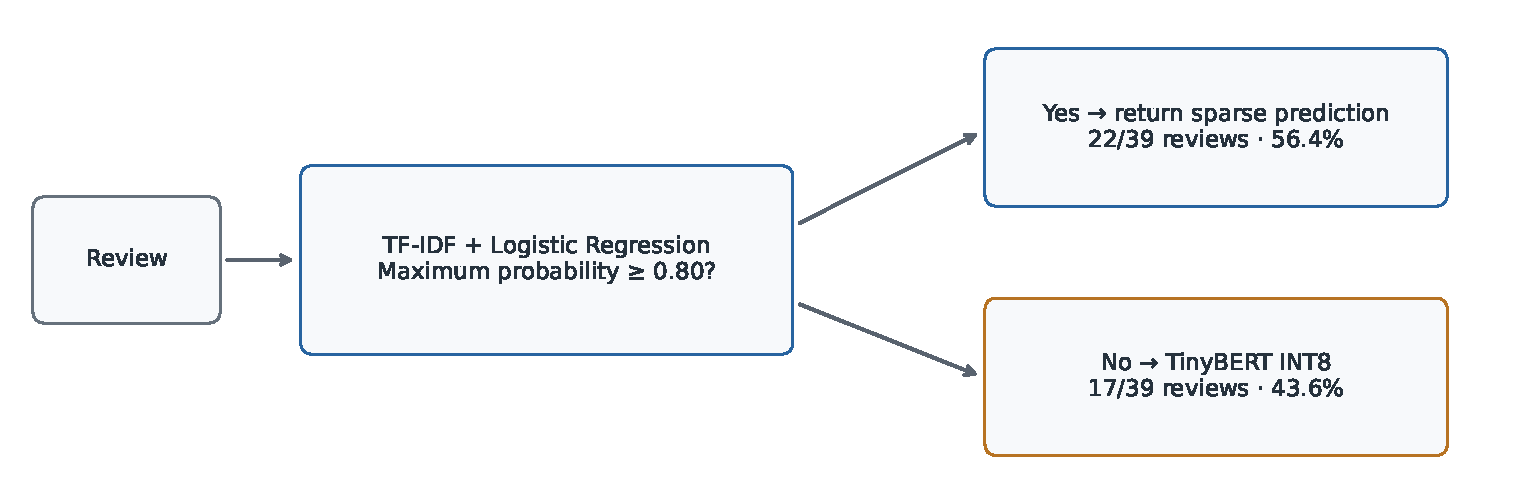
\includegraphics[width=0.72\linewidth]{cascade_diagram}
  \caption{Cascade classifier routing logic. An input is first processed by
    Logistic Regression; if the predicted class probability meets the
    confidence threshold $\tau$, its prediction is returned directly (fast
    path); otherwise TinyBERT INT8 is queried (fallback path).}
  \label{fig:cascade_diagram}
\end{figure}

\textbf{Hardness.}  Sentiment classification is non-trivial whenever reviews use
negation, sarcasm, or mixed sentiment.  For linear models, the fundamental
difficulty is representational: a vocabulary of size $d$ admits $O(d^2)$
pairwise feature interactions, but a linear decision boundary in $\mathbb{R}^d$
assigns a fixed coefficient to each unigram or bigram feature. Bigrams encode
limited adjacent-word information, but the model lacks broader contextual
representations.  Transformer models address this via self-attention, but
their non-linear decision functions are harder to inspect directly. Here we
use post-hoc local approximation as one available explanation route.  The cascade further complicates
interpretability: the applicable explanation method depends on which component
handled each input, making the system a mixture model in both prediction and
explanation.

\textbf{Metrics.}  We evaluate accuracy, binary F1, precision, recall,
and average per-sample inference time (ms) under identical CPU conditions.

\textbf{Explainability.}  For $f_1$ we inspect the learned weight vector
$\mathbf{w}$ globally.  For local explanations we apply
LIME~\citep{ribeiro2016} to both $f_1$ and $f_2$: given input $x$, LIME fits a
sparse linear model $h$ over perturbed neighbours $\mathcal{N}(x)$, minimising
\[
  \sum_{z \in \mathcal{N}(x)} \pi_x(z)\,(f(z) - h(z))^2 + \Omega(h).
\]
Integrated Gradients~\citep{sundararajan2017} was planned for $f_2$ but was not
run because the repository retained only a quantized checkpoint rather than a
float model suitable for gradient attribution.  LIME therefore serves as a
model-agnostic fallback throughout.


% ----------------------------------------------------------
\section{Related Work}
% ----------------------------------------------------------

\textbf{Post-hoc local explanations.}  \citet{ribeiro2016} introduced LIME,
which approximates a complex classifier locally via a sparse linear model fitted
over perturbed inputs; it is model-agnostic but can vary between runs due to
stochastic sampling.  \citet{lundberg2017} proposed SHAP, grounding feature
attributions in Shapley values from cooperative game theory. SHAP was not
applied in this project; learned coefficients and feature-value-weighted
contributions were used for the linear model.

\textbf{Attribution for neural networks.}  \citet{sundararajan2017} introduced
Integrated Gradients, which integrates gradients along a path from a baseline
to the input and satisfies an implementation invariance axiom; the method
requires an appropriate differentiable model path. The retained quantized
checkpoint did not provide a compatible path for our planned implementation.

\textbf{Attention as explanation.}  \citet{jain2019} showed that attention
weights do not reliably correspond to other measures of feature importance;
\citet{wiegreffe2019} challenged this finding; and \citet{serrano2019} found
that attended tokens are not always causally responsible for model outputs.
Collectively, these results suggest attention is an unreliable explanation
source.

\textbf{Cross-family interpretability.}  Most prior work studies individual
model types or explanation methods in isolation.  This project addresses that
gap by comparing sparse linear classifiers, a compact quantized transformer,
and a cascade system, focusing on how architecture and efficiency constraints
shape interpretability.


% ----------------------------------------------------------
\section{Methodology}
% ----------------------------------------------------------

\textbf{Dataset and preprocessing.}  We use the IMDb Large Movie Review Dataset.
For the sparse baseline, each review is represented as a TF-IDF weighted vector
over unigrams and bigrams (n-gram range 1--2) using scikit-learn.  The active
pipeline lowercases text, removes English stop words, and keeps terms appearing
in at least two training documents.  TF-IDF weighting surfaces evaluative
vocabulary by downweighting corpus-wide frequent terms.

\textbf{Logistic Regression ($f_1$).}  Trained on the TF-IDF representation
with L2 regularisation.  The learned weight vector provides a direct global
explanation: terms with large positive weights indicate positive sentiment and
vice versa.

\textbf{TinyBERT INT8 ($f_2$).}  We use TinyBERT \citep{jiao2020}, a
four-layer transformer obtained by knowledge distillation from BERT-base,
making it substantially smaller and faster than its teacher while retaining
much of its representational capability.  TinyBERT was fine-tuned on the
training set for sentiment classification and subsequently post-training
dynamically quantized to INT8 for its linear layers. A memory comparison
was not measured. Only the quantized fine-tuned checkpoint was retained, so
the planned gradient-attribution path was not run.

\textbf{Cascade classifier ($f_3$).}  Logistic Regression is queried first; the
maximum predicted class probability is used as a routing score.  If
$c(x) \geq \tau$ the cascade returns $f_1$'s prediction; otherwise it queries
$f_2$.  This keeps the routing criterion directly interpretable and tied to the
actual classifier probabilities rather than an external heuristic.

\textbf{Explainability pipeline.}  For $f_1$ we extract the top-ranked positive
and negative feature weights globally. Coefficients are fixed for a retained
model, but stability across retraining was not evaluated.  For both $f_1$ and $f_2$ we apply LIME to a
small illustrative set drawn from the first five rows of the clean evaluation
sample. LIME describes local responses to word perturbations; its outputs
can differ from global coefficients and can vary between runs.  Integrated Gradients (planned for
$f_2$) was not feasible in the final repository because only the quantized
checkpoint was retained.


% ----------------------------------------------------------
\section{Experimental Setup}
% ----------------------------------------------------------

\textbf{Evaluation sample.}  Final evaluation uses a small clean sample derived
from an original 100-row candidate CSV by removing every review whose text
appears exactly in the training file, then dropping duplicate texts inside the
remaining sample.  This leaves 39 labelled examples.  The local training CSV contains 30,000 reviews, balanced across labels.
Exactly 61 candidate rows overlap its raw review text; no additional
duplicates remain after exclusion. This custom project partition is not the
official IMDb 25,000-review test split. The split-creation logic is saved in
a short script, and file hashes record the input identities.  Because the resulting sample is
small, all quantitative differences should be treated as indicative rather than
statistically reliable.

\textbf{Evaluation metrics.}  For each model we report accuracy, binary F1,
precision, recall, and average wall-clock inference time per sample (ms)
over the full evaluation sample.  Precision and recall are reported separately because
the two main model families exhibit distinct error profiles.

\textbf{Hardware.}  All models were evaluated on CPU without GPU acceleration,
consistent with the project's focus on resource-constrained deployment.  No
cross-validation was performed, as the primary goal is comparative explanation
analysis rather than exhaustive model optimisation.

\textbf{Timing protocol.}  To keep latency comparisons fair, all three models
are timed in the same per-sample prediction loop on CPU.  Each evaluation is
repeated three times and the average wall-clock time is reported.

\textbf{Cascade threshold.}  We use a single probability threshold
$\tau = 0.80$ for the final cascade.  No threshold sweep is claimed in the
final analysis.

\textbf{Explainability evaluation.}  The analysis is primarily qualitative.
We examine global feature weights for the linear models and LIME explanations
on the first five rows of the clean evaluation sample.  A formal stability
analysis or large-scale quantitative
comparison is not conducted; the evaluation sample is too small for statistically
meaningful conclusions of that kind.


% ----------------------------------------------------------
\section{Results}
\label{sec:results}
% ----------------------------------------------------------


\subsection{Quantitative Performance}

Table~\ref{tab:performance} summarises classification performance and inference
time on the clean evaluation sample.

\begin{table}[ht]
\centering
\caption{Classification performance and inference time on the clean evaluation
sample ($n=39$). Speedup is relative to TinyBERT INT8.}
\label{tab:performance}
\setlength{\tabcolsep}{5pt}
\begin{tabular}{lrrrrrl}
\toprule
Model & Acc. & F1 & Prec. & Recall & ms/samp. & Speedup \\
\midrule
TF-IDF + LR   & 0.974 & 0.973 & 1.000 & 0.947 & 0.28 & 35.3$\times$ \\
TinyBERT INT8 & 0.923 & 0.919 & 0.944 & 0.895 & 9.88 & 1$\times$  \\
Cascade ($\tau{=}0.80$) & 0.949 & 0.944 & 1.000 & 0.895 & 5.19 & 1.91$\times$ \\
\bottomrule
\end{tabular}
\end{table}

\begin{figure}[ht]
  \centering
  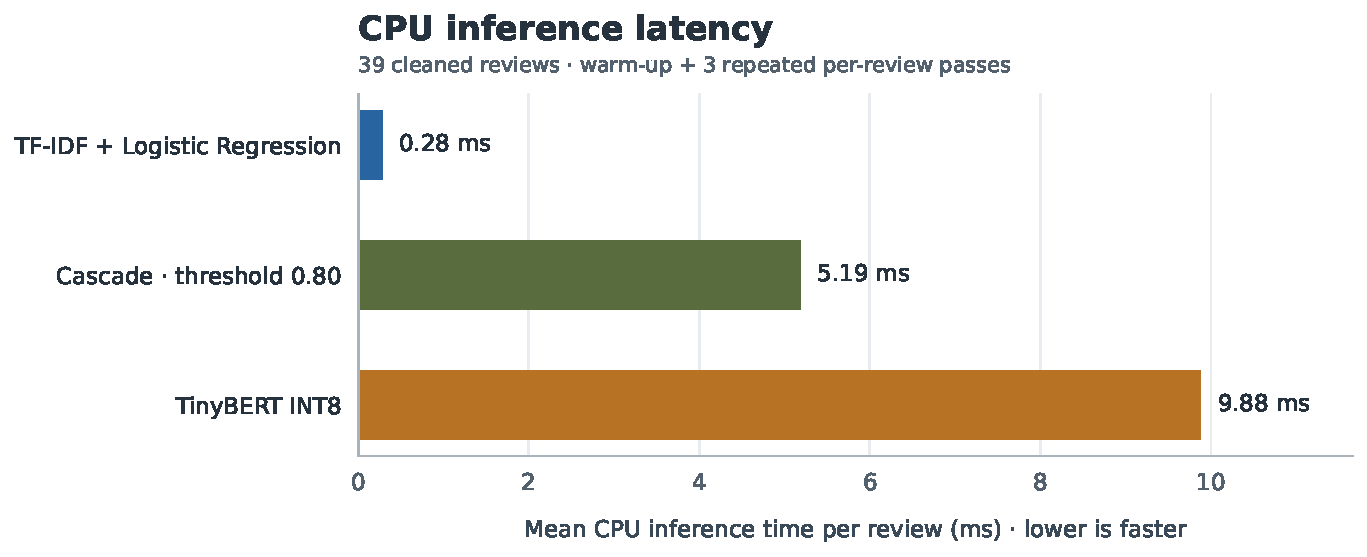
\includegraphics[width=0.72\linewidth]{latency}
  \caption{Average inference latency per sample on CPU. Logistic Regression is
    approximately 35$\times$ faster than TinyBERT INT8 on the final clean
    evaluation sample ($n{=}39$, $\tau{=}0.80$). The figure is generated
    directly from the saved clean evaluation JSON used by Table~\ref{tab:performance}.}
  \label{fig:latency}
\end{figure}

On the clean evaluation sample, TF-IDF + Logistic Regression achieves the best
predictive result: 38 correct predictions out of 39, with accuracy 97.4\%,
precision 1.00, recall 0.947, and binary F1 0.973.  TinyBERT INT8 reaches
92.3\% accuracy and F1 0.919, while the cascade sits between the two at 94.9\%
accuracy and F1 0.944.  Because the clean sample is so small, these differences
should still be read cautiously; they are based on only one or two reviews.

The clearest quantitative difference is still efficiency.  Logistic Regression
runs at 0.28~ms per sample, compared with 9.88~ms for TinyBERT INT8
a gap of roughly 35$\times$ under the shared timing setup.  The cascade at
$\tau = 0.80$ averages 5.19~ms, reflecting the fact
that it can keep part of the traffic on the sparse model while still falling
back to TinyBERT when Logistic Regression is uncertain.


\subsection{Cascade Routing Behaviour}

At $\tau = 0.80$, the cascade routed 22 of the 39 clean evaluation examples
(56.4\%) to Logistic Regression and 17 (43.6\%) to TinyBERT.  On this sample
it improves on TinyBERT's latency while also improving on TinyBERT's accuracy,
but it does not match the sparse model's best result.  This does not prove that
the cascade is universally superior; on such a small sample it simply shows
that a basic probability gate can recover some of the sparse model's speed
while keeping predictive performance in the same range.

\begin{table}[ht]
\centering
\caption{Observed cascade routing at the single threshold used in the final
analysis.}
\label{tab:cascade}
\setlength{\tabcolsep}{5pt}
\begin{tabular}{crrrr}
\toprule
$\tau$ & LR routed & BERT routed & Accuracy & ms/samp. \\
\midrule
\textbf{0.80} & \textbf{56.4\%} & \textbf{43.6\%} & \textbf{94.9\%} & \textbf{5.19} \\
\bottomrule
\end{tabular}
\end{table}

\begin{figure}[ht]
  \centering
  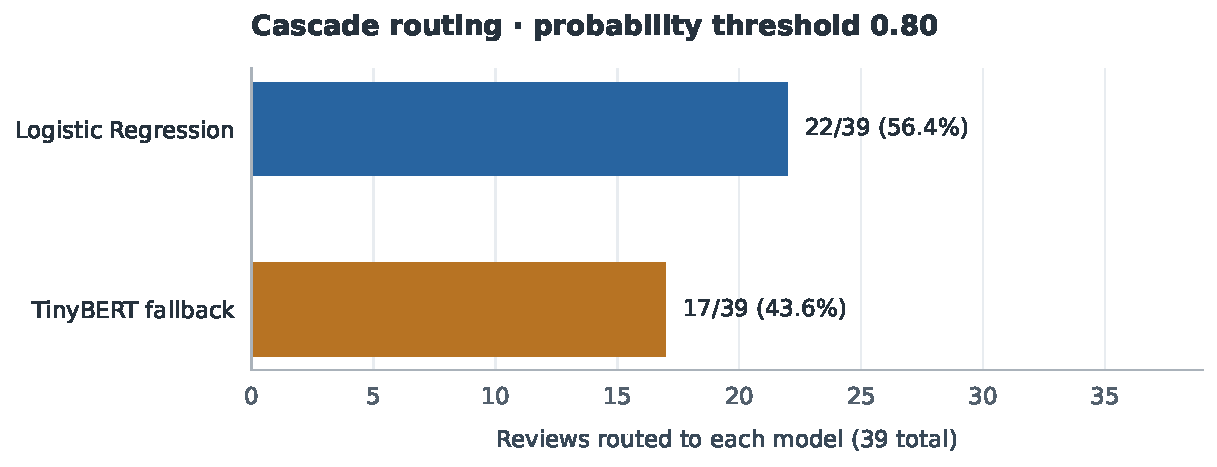
\includegraphics[width=0.72\linewidth]{cascade_routing}
  \caption{Cascade routing on the 39-review clean evaluation sample at
    $\tau{=}0.80$: 22 reviews (56.4\%) used Logistic Regression, and
    17 reviews (43.6\%) used TinyBERT.}
  \label{fig:cascade_routing}
\end{figure}

The routing interpretation is straightforward because the gate is based on
Logistic Regression probabilities rather than a hand-designed confidence score.
That makes the final cascade section easier to defend, even though the result
still rests on a very small evaluation sample.


\subsection{Global Explanation Analysis}

\begin{figure}[ht]
  \centering
  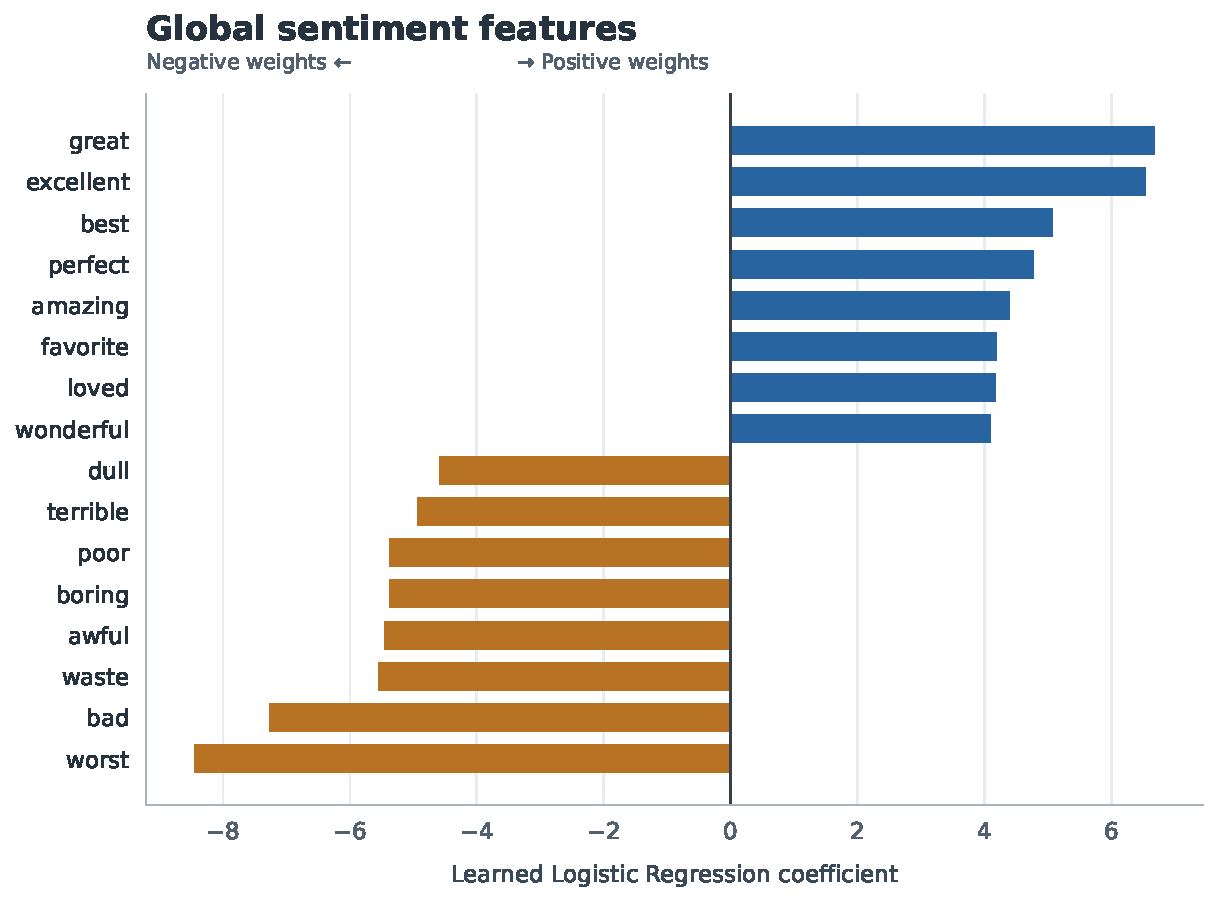
\includegraphics[width=0.72\linewidth]{feature_weights}
  \caption{Top positive and negative feature weights learned by TF-IDF +
    Logistic Regression.  Blue bars indicate terms associated with positive
    sentiment; orange bars indicate terms associated with negative sentiment.}
  \label{fig:lr_weights}
\end{figure}

Inspecting the top-ranked feature weights of the Logistic Regression model
reveals a pattern closely resembling a manually constructed sentiment lexicon.
The most negatively weighted terms include
\emph{worst}, \emph{bad}, \emph{waste}, \emph{boring}, and \emph{awful};
the most positively weighted include \emph{excellent}, \emph{great},
\emph{amazing}, and \emph{brilliant}.  This is consistent with what one would
expect from a model trained on a sentiment benchmark with clear evaluative
language.
These coefficients expose learned lexical associations. Bigrams provide
some adjacent-word information, while longer-range interactions are absent.  Some weights are less
interpretable -- words such as \emph{today} and \emph{minutes} appear with
non-trivial weights, likely reflecting dataset artefacts (co-occurrence with
phrases like \emph{waste of two minutes}) rather than genuine sentiment signal.
No causal error study of these features was performed. They illustrate why
a learned coefficient should be interpreted as a model association, rather
than as an independently verified sentiment rule.


\subsection{Local Explanation Analysis}

\begin{figure}[ht]
  \centering
  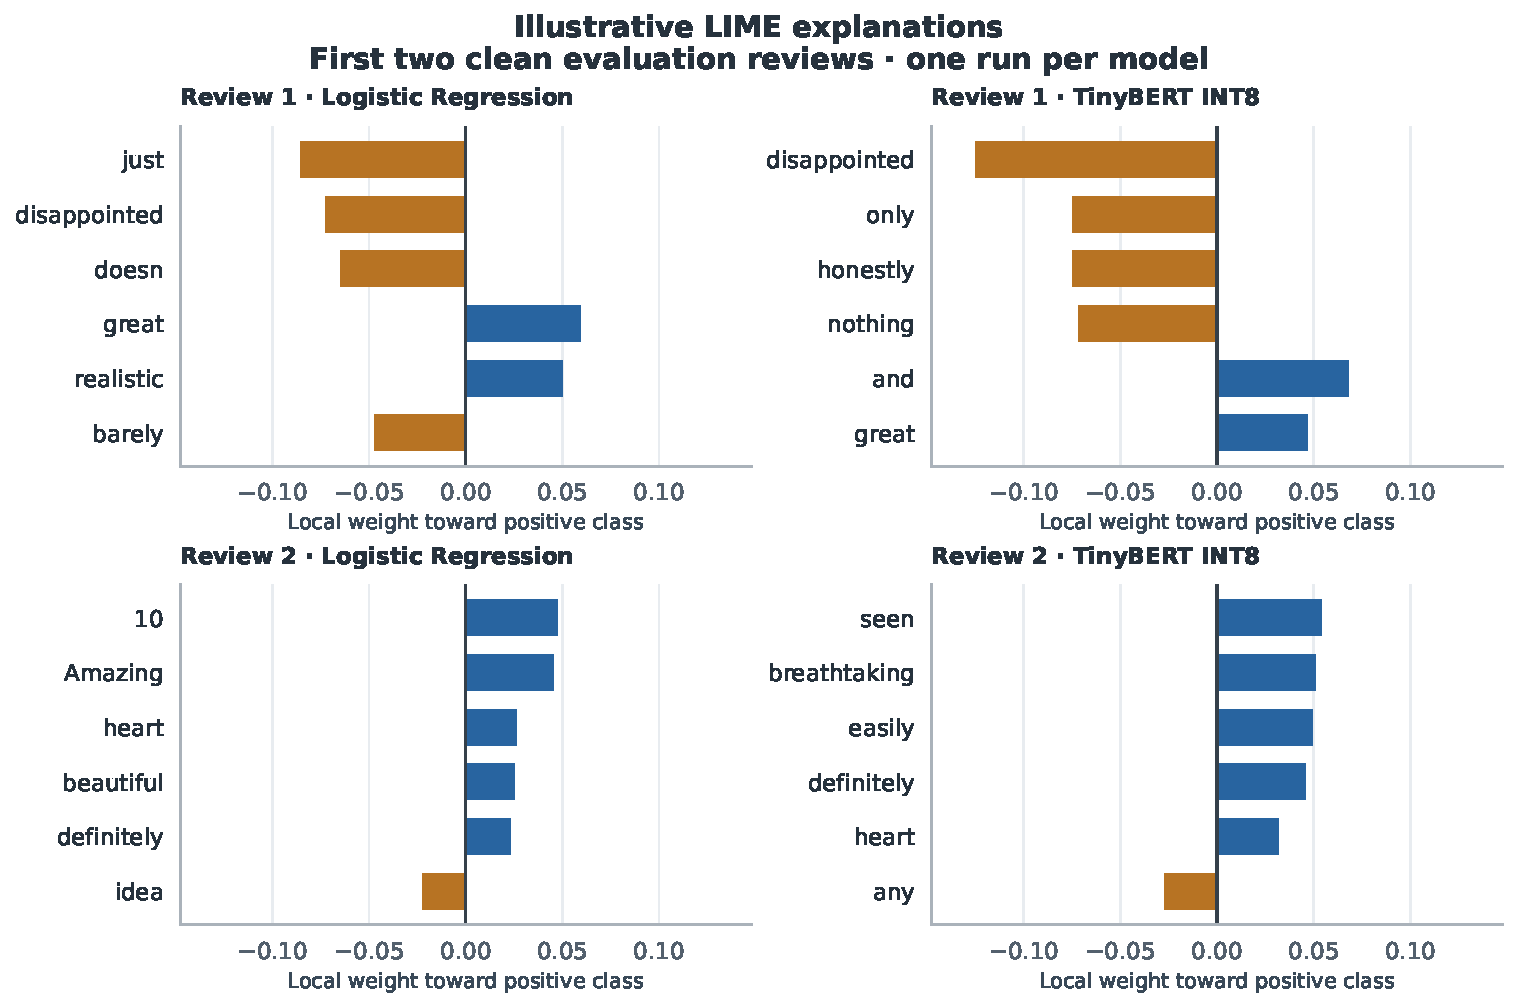
\includegraphics[width=\linewidth]{lime_examples}
  \caption{LIME local explanations for the first two clean evaluation reviews.
    Both columns use the same horizontal scale. Blue weights support the
    positive class and orange weights oppose it. These saved runs illustrate
    local perturbation responses; they do not establish explanation stability
    or a causal account of model reasoning.}
  \label{fig:lime}
\end{figure}

LIME explanations were computed for the first five rows of the clean evaluation
sample. All five are retained in each model's saved JSON output; the figure
shows the first two. The examples are illustrative and were not selected as a
representative evaluation of explanation quality.

\textbf{Example 1.} Both models predict negative sentiment. The token
\emph{disappointed} has negative LIME weight for both models, while
\emph{great} has positive weight. Their other highly ranked terms differ:
Logistic Regression emphasizes \emph{just}, while TinyBERT includes
\emph{only} and \emph{honestly} among its negative weights.

\textbf{Example 2.} Both models predict positive sentiment. Logistic Regression
assigns positive local weight to \emph{Amazing} and \emph{beautiful};
TinyBERT assigns positive weight to \emph{breathtaking} and \emph{easily}.
Both give positive weight to \emph{heart} and \emph{definitely}.

These are descriptions of saved surrogate-model coefficients. Differences in
word rankings do not by themselves prove that TinyBERT resolves context more
faithfully. LIME is stochastic, and neither repeated-seed stability nor
explanation faithfulness was evaluated.


\subsection{Failure Cases and Limitations of Explanation Methods}

The saved aggregate metrics show one error for Logistic Regression, three for
TinyBERT, and two for the cascade. They do not identify which review belongs to
each cross-model error category. We therefore do not attribute a specific
sarcasm or negation failure to these aggregate results.

A future error analysis should retain per-review predictions and compare
negation, mixed sentiment, long reviews, and ambiguous phrasing on a larger
independent sample. It should distinguish actual observed errors from examples
constructed to illustrate an architectural limitation.

\textbf{Limitations of explanation methods.}  The most significant constraint
is that Integrated Gradients was not run for TinyBERT because the repository
retained only a quantized checkpoint.  This should not be phrased as a general
claim that INT8 models can never support gradient-based XAI; the narrower point
is that saving only the quantized artifact removed that option in this project.
Saving a float32 checkpoint before quantization would preserve the ability to
run gradient-based attribution later.


% ----------------------------------------------------------
\section{Conclusions}
% ----------------------------------------------------------

This project investigated how accuracy, efficiency, and interpretability
interact across three sentiment classification systems.  Evaluation was
conducted on a small clean sample of 39 examples created by removing exact
train-set overlap from an original 100-row candidate file; stronger conclusions
would require a substantially larger evaluation.

On performance, Logistic Regression gives the strongest result on this clean
sample and remains dramatically faster on CPU.  Because the sample contains
only 39 rows, that should still be framed cautiously; the most reliable
conclusion is about the large efficiency gap, not about a decisive accuracy
ordering between model families.

On interpretability, the retained sparse model offers inspectable global
feature weights that reveal lexical sentiment associations.  TinyBERT required model-agnostic local
explanations, and those LIME plots are useful only as qualitative diagnostics.
The cascade with $\tau = 0.80$ shows that a simple probability gate can reduce
latency relative to TinyBERT alone while preserving most of the sparse model's
performance on this small sample.

The unavailability of Integrated Gradients reflects a practical repository
constraint: retaining only a quantized checkpoint prevented gradient-based XAI
analysis in the final submission.  Saving a float32 checkpoint before
quantization would preserve that option, with an additional model-storage requirement.

\textbf{Future work.}  Evaluation on a substantially larger test set would
enable reliable statistical comparisons and explanation stability analysis.
Retaining a float32 TinyBERT checkpoint before quantization would allow
Integrated Gradients to be applied, enabling a principled comparison between
gradient-based and perturbation-based explanations.


% ----------------------------------------------------------
% References
% ----------------------------------------------------------

\begin{thebibliography}{8}

\bibitem[Jain and Wallace(2019)]{jain2019}
Sarthak Jain and Byron~C. Wallace.
\newblock Attention is not explanation.
\newblock In \emph{Proceedings of the 2019 Conference of the North American
  Chapter of the Association for Computational Linguistics: Human Language
  Technologies (NAACL-HLT)}, pages 3543--3556, 2019.

\bibitem[Jiao et al.(2020)]{jiao2020}
Xiaoqi Jiao, Yichun Yin, Lifeng Shang, Xin Jiang, Xiao Chen, Linlin Li,
  Fang Wang, and Qun Liu.
\newblock {TinyBERT}: Distilling {BERT} for natural language understanding.
\newblock In \emph{Findings of the Association for Computational Linguistics:
  EMNLP 2020}, pages 4163--4174, 2020.

\bibitem[Maas et al.(2011)]{maas2011}
Andrew~L. Maas, Raymond~E. Daly, Peter~T. Pham, Dan Huang, Andrew~Y. Ng, and
  Christopher Potts.
\newblock Learning word vectors for sentiment analysis.
\newblock In \emph{Proceedings of the 49th Annual Meeting of the Association
  for Computational Linguistics (ACL)}, pages 142--150, 2011.

\bibitem[Lundberg and Lee(2017)]{lundberg2017}
Scott~M. Lundberg and Su-In Lee.
\newblock A unified approach to interpreting model predictions.
\newblock In \emph{Advances in Neural Information Processing Systems~30
  (NeurIPS)}, pages 4766--4777, 2017.

\bibitem[Ribeiro et al.(2016)]{ribeiro2016}
Marco~Tulio Ribeiro, Sameer Singh, and Carlos Guestrin.
\newblock ``{Why Should I Trust You?}'': Explaining the predictions of any
  classifier.
\newblock In \emph{Proceedings of the 22nd ACM SIGKDD International Conference
  on Knowledge Discovery and Data Mining (KDD)}, pages 1135--1144, 2016.

\bibitem[Serrano and Smith(2019)]{serrano2019}
Sofia Serrano and Noah~A. Smith.
\newblock Is attention interpretable?
\newblock In \emph{Proceedings of the 57th Annual Meeting of the Association
  for Computational Linguistics (ACL)}, pages 2931--2951, 2019.

\bibitem[Sundararajan et al.(2017)]{sundararajan2017}
Mukund Sundararajan, Ankur Taly, and Qiqi Yan.
\newblock Axiomatic attribution for deep networks.
\newblock In \emph{Proceedings of the 34th International Conference on Machine
  Learning (ICML)}, pages 3319--3328, 2017.

\bibitem[Wiegreffe and Pinter(2019)]{wiegreffe2019}
Sarah Wiegreffe and Yuval Pinter.
\newblock Attention is not not explanation.
\newblock In \emph{Proceedings of the 2019 Conference on Empirical Methods in
  Natural Language Processing and the 9th International Joint Conference on
  Natural Language Processing (EMNLP-IJCNLP)}, pages 11--20, 2019.

\end{thebibliography}

\end{document}
